\label{sec:introduction}
Missing data remains a persistent obstacle in scientific and public-health analysis. In county-level surveillance, privacy suppression and sparse reporting are not random: missing entries often cluster in low-count regions, which can bias downstream trend analysis and resource allocation if imputed poorly. At the same time, many applied workflows treat imputation as a black-box preprocessing step and provide limited tools to compare methods or inspect why a value was imputed in a particular way.

We present \tool, a visual analytics dashboard that supports the full imputation workflow: diagnosing missingness, selecting and tuning models, comparing outcomes, and inspecting provenance. The system integrates common imputers (MICE, Random Forest, XGBoost, linear/kNN baselines) and a geospatially informed method (\gknn) that blends socioeconomic and spatial distance. Rather than promoting one model universally, \tool is designed to make method choice auditable through linked visual diagnostics and quantitative summaries.

Our contributions are threefold: (1) a method-agnostic visual analytics workflow for missingness diagnosis and post-imputation comparison; (2) a modular benchmarking backend with cached runs and consistent holdout-based evaluation; and (3) \gknn, a geographically informed kNN variant with donor-level provenance that can be interrogated directly in the interface.

\begin{figure*}[t]
  \centering
  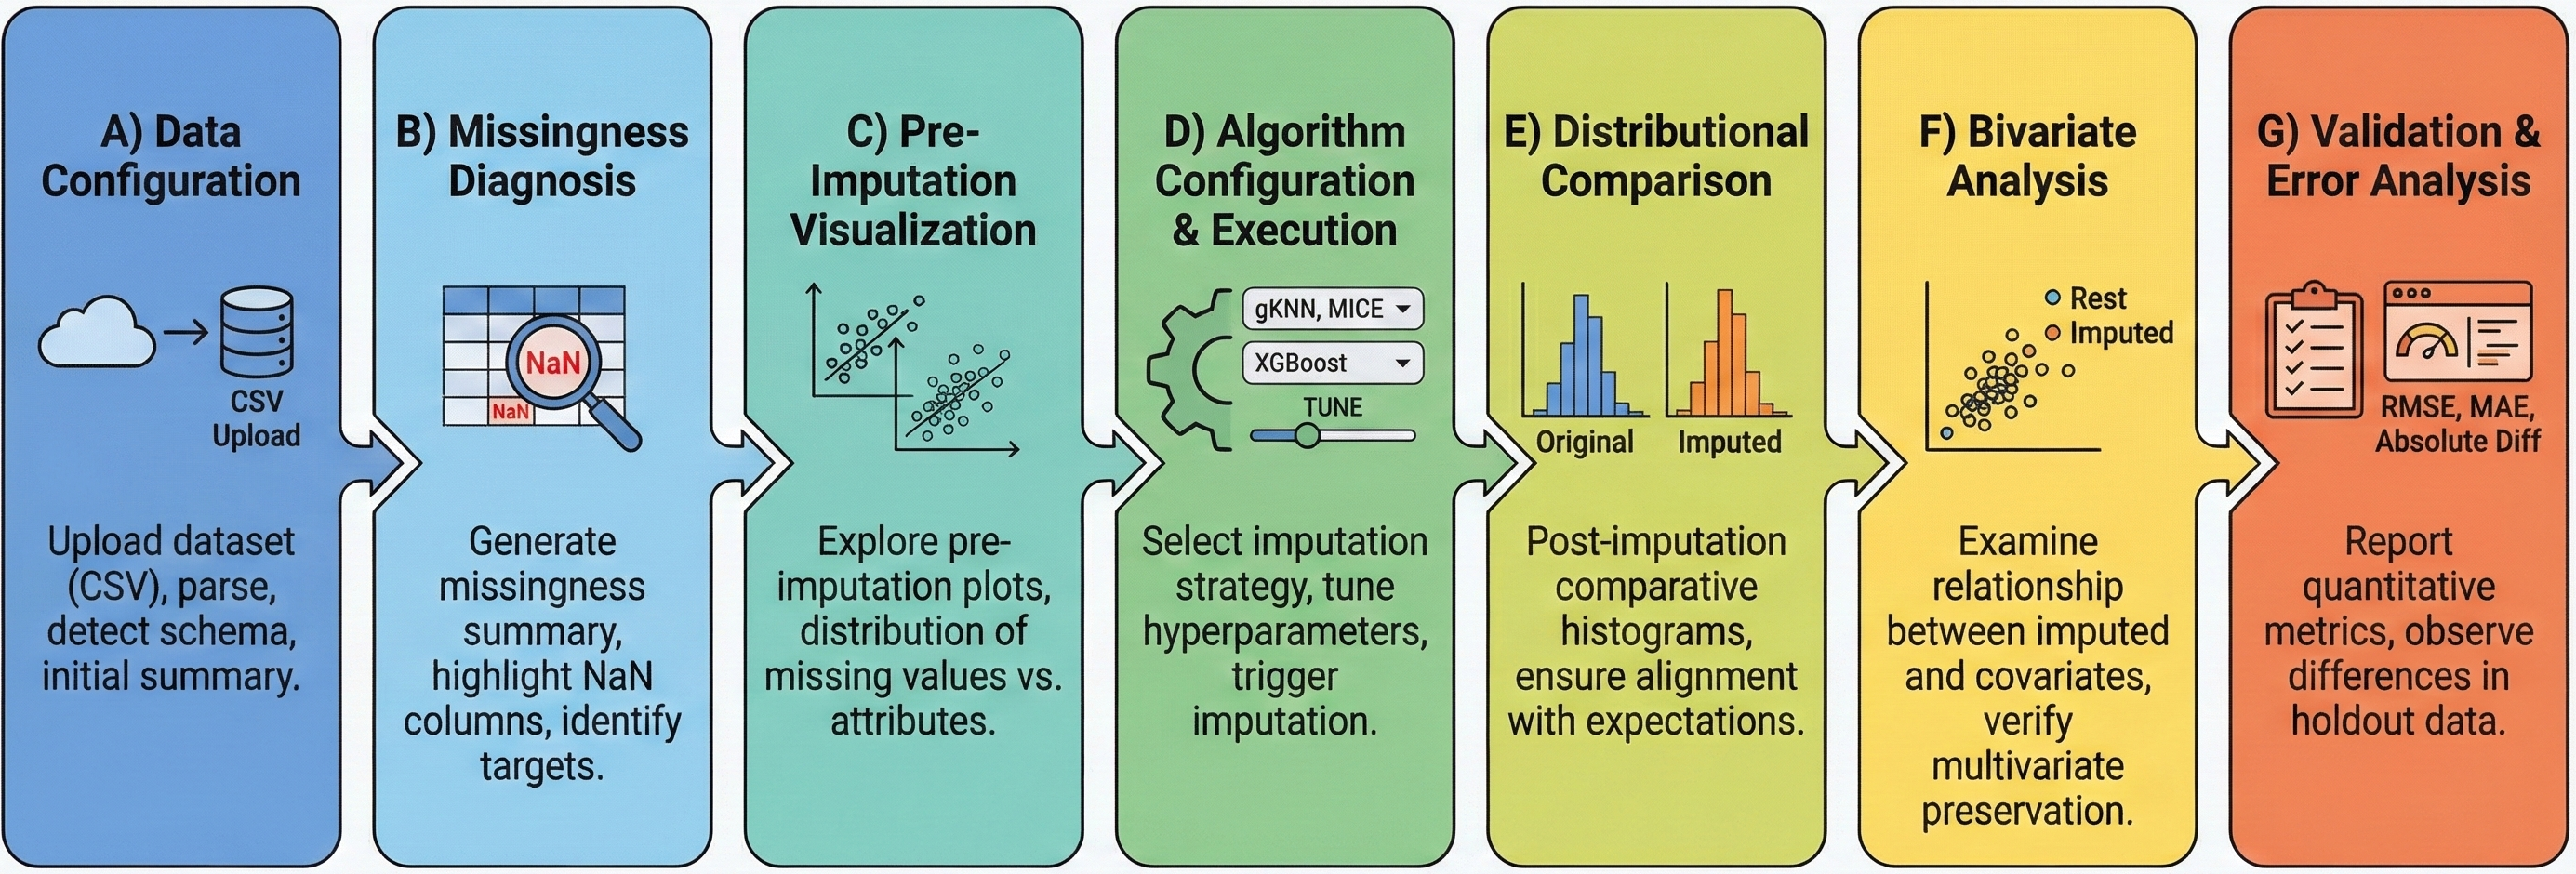
\includegraphics[width=0.93\linewidth]{user_flow.png}
  \caption{Figure: Seven-stage \tool workflow from data upload and missingness diagnosis to model execution, visual comparison, and validation.}
  \label{fig:workflow_short}
\end{figure*}

\section{Related Work}
\paragraph*{Imputation methods.}
Imputation approaches include chained equations (MICE), tree ensembles, and instance-based methods~\cite{VanBuuren2018MICE,Breiman2001RandomForest,Chen2016XGBoost,Cover1967KNN}. Spatial extensions of nearest-neighbor imputation can better exploit locality when outcomes are geographically autocorrelated~\cite{baker2014missing}. Our \gknn builds on this line with a weighted blend of socioeconomic and geographic distance learned via Bayesian optimization~\cite{snoek2012practical}.

\paragraph*{Visual analytics and uncertainty.}
Visual analytics research emphasizes integrating computational models with interactive reasoning~\cite{Endert2017}. Prior systems support health-data exploration and uncertainty communication~\cite{sankaran2016opioid,Carroll2014HealthVis,Sacha2016UncertaintyTrust}, but many operate on precomputed outputs. \tool instead couples model execution with linked diagnostics so analysts can compare methods within a single iterative loop.

\section{Data and Design Goals}
\paragraph*{Datasets.}
We evaluate on two datasets. First, county-level U.S.\ prescription-opioid mortality (2000--2022) from CDC WONDER~\cite{cdcWonderDrugPoisoning}, joined with ACS socioeconomic covariates~\cite{acsPopulation} and county geometries~\cite{tigerShapefiles}. Missingness is structured rather than MCAR because suppression concentrates in low-count counties and often forms spatial clusters. Second, a non-geographic telecom churn dataset~\cite{telcoHF} (212 rows after filtering), where we impute the continuous \texttt{Offer} target from numeric covariates.

\section{Design Goals}
From analyst feedback, we target four design goals that guided both algorithm integration and interface decisions.

\paragraph*{DG1: Make missingness legible.}
Analysts need immediate visibility into where missing values occur, whether they cluster by feature or region, and whether missingness correlates with plausible covariates. The system therefore prioritizes missingness summaries and pre-imputation relationship views before any model execution.

\paragraph*{DG2: Enable fair, model-agnostic comparison.}
Method choice should be driven by evidence rather than familiarity. To support this, all models are run under consistent masks and feature handling, and results are summarized with comparable metrics (MAE, RMSE, \(\Delta\)RMSE, runtime) for the current target and regime.

\paragraph*{DG3: Support visual plausibility checks.}
Aggregate error alone can hide local artifacts. Linked scatterplots and histograms with stable axis scales let analysts inspect whether imputations preserve relationships, distort tails, or introduce implausible clusters when switching algorithms.

\paragraph*{DG4: Preserve provenance and spatial interpretability.}
For geographically structured data, users must inspect who contributed to an imputed value. The map and donor inspection views therefore expose donor counties and context so analysts can verify neighborhood effects and borrowing plausibility.

Together, these goals frame imputation as an analytic reasoning problem rather than only a predictive task. In practice, users alternate between checking model scores and visually validating whether local behavior matches domain expectations. The interface is therefore designed to keep diagnostics and evidence co-located, reducing mode switching between separate scripts, notebooks, and reporting tools.

\section{Methodology and System Design}
\paragraph*{Architecture and workflow.}
\tool uses a Python/FastAPI backend and React/TypeScript frontend. The backend manages sessions, profiles missingness, runs imputers, and caches results by session/method/target/mask; the frontend links configuration, diagnostics, distribution views, and method-comparison panels for rapid iterative analysis (Figure~\ref{fig:workflow_short}).

\paragraph*{Imputation models.}
We include linear regression, non-spatial kNN, Random Forest, XGBoost, MICE (IterativeImputer with ridge chains), and \gknn. For \gknn, we compute socioeconomic and geographic distance matrices and optimize blending weight \(\alpha\) and neighborhood size \(k\):
\begin{equation}
  D_{\text{blend}}=\alpha D_{\text{socio}}+(1-\alpha)D_{\text{geo}}.
\end{equation}
Masked counties are imputed by inverse-distance weighted donor averages, and donor sets are retained for visual provenance inspection.

\paragraph*{Evaluation protocol.}
For each selected target, we apply a 20\% holdout mask on observed values and run each algorithm under identical conditions. We report MAE, RMSE, \(\Delta\)RMSE, and runtime in a unified comparison table. Additional suppression-like and intermediate masking presets probe more structured missingness regimes. We also compute paired Wilcoxon signed-rank tests offline and run a copula-based uncertainty analysis for \gknn~\cite{nelsen2006introduction,joe2014dependence,hollenbach2021multiple}.

\paragraph*{System design rationale.}
The dashboard is organized around iterative analyst behavior rather than a single linear pipeline: users repeatedly switch targets, rerun methods, and revisit comparisons as hypotheses evolve. Caching and synchronized state were therefore prioritized to keep this loop interactive. The design intentionally pairs numeric summaries with linked views so that method rankings can be interpreted with visual evidence rather than treated as final in isolation.

\subsection{Design process and requirements}
The system design was shaped through iterative feedback from data-analysis users in an academic public-health context. Early sessions revealed fragmented workflows in which missingness diagnosis, model execution, and plausibility checking were handled in separate tools. This motivated a unified interface where diagnosis, benchmarking, and provenance inspection are tightly connected.

Three requirements drove implementation priorities: (R1) algorithmic versatility across spatial and non-spatial imputers; (R2) consistent quantitative evaluation under shared masking settings; and (R3) interpretable outputs that expose donor-level context and cross-method differences. These requirements map directly to the dashboard organization and to backend decisions such as per-configuration caching and standardized metric reporting.

\section{Backend Imputation Framework}
\paragraph*{Backend imputation framework.}
The backend exposes endpoints for upload, profiling, imputation, evaluation, and export. Profiles include null percentages, co-missingness structure, and candidate target identification; these summaries populate early-stage diagnostic views before any method is executed. Completed runs are keyed by dataset, target, algorithm, and mask parameters, which avoids recomputation and allows rapid cross-method switching during exploratory sessions.

\paragraph*{Front-end visual analytics design.}
The front end emphasizes coherence across linked views. Method selection in the comparison table updates all downstream visualizations, and axis domains remain fixed across methods for direct pattern comparison. This choice addresses a frequent analyst complaint in earlier prototypes: inconsistent scales made it hard to distinguish true model differences from visual rescaling artifacts.

\begin{figure*}[t]
  \centering
  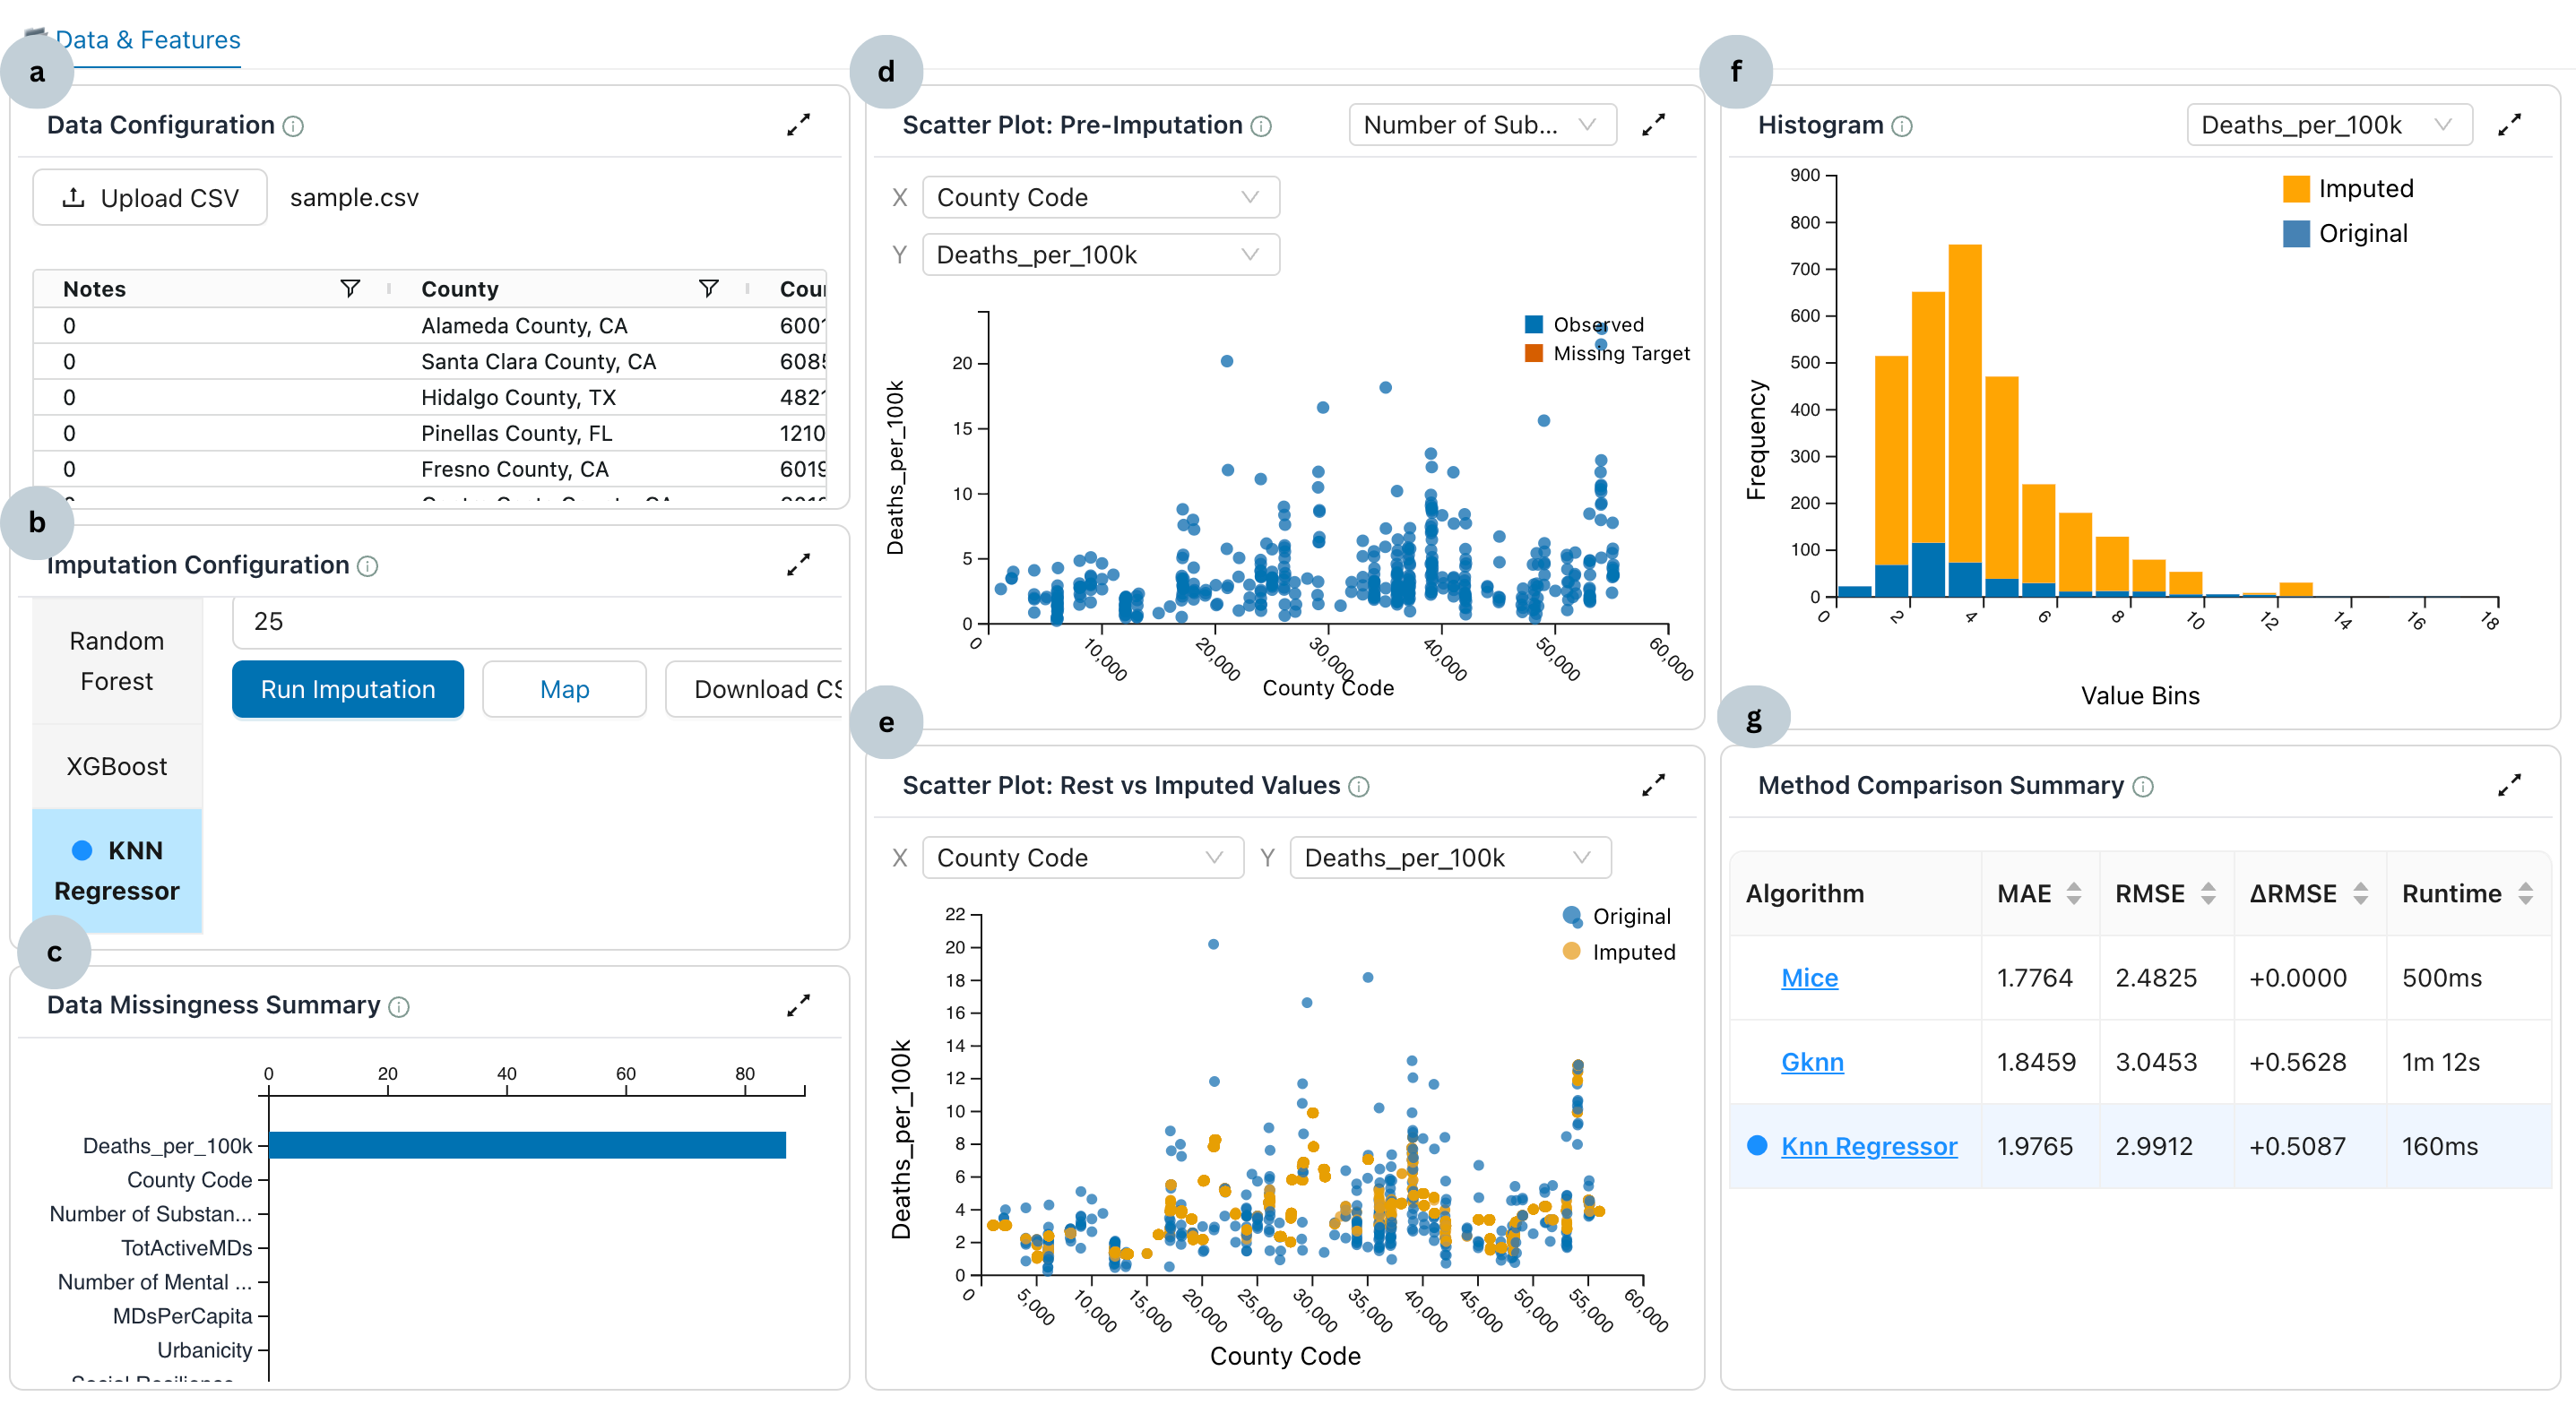
\includegraphics[width=\linewidth]{Dashboard_new.png}
  \caption{Figure: \tool dashboard with linked panels for data configuration, missingness summary, pre/post-imputation plots, and cross-method evaluation.}
  \label{fig:dashboard_short}
\end{figure*}

\section{Front-End Visual Analytics}
The front end exposes seven coordinated panels (Figure~\ref{fig:dashboard_short}) that align with the end-to-end analyst workflow. Users begin with data and imputation configuration, then inspect missingness and pre-imputation relationships to hypothesize mechanisms (e.g., MCAR/MAR/MNAR). After model execution, linked scatterplots and histograms compare observed versus imputed values under fixed axes, reducing cognitive load when switching methods. The method-comparison panel summarizes MAE, RMSE, \(\Delta\)RMSE, and runtime for all executed methods under the same mask.

For spatial datasets, a geomap view supports donor-level explanation. Selecting an imputed county highlights donor counties and exposes their contributions, enabling analysts to verify whether borrowing patterns are geographically and socioeconomically plausible.

\paragraph*{Panel interactions.}
The Data Configuration and Imputation Configuration panels define the active target and method context used throughout the interface. Missingness summaries and pre-imputation views help analysts choose suitable targets and predictors before launching runs. Post-imputation panels then provide complementary checks: scatterplots reveal relationship preservation, histograms reveal marginal shifts, and the comparison table provides rankable quantitative evidence for method choice.

\paragraph*{Cross-view coordination.}
All panels share a synchronized state. Choosing a method in the comparison table immediately updates post-imputation plots and map overlays. This linked behavior supports rapid what-if analysis and reduces context switching between separate tools. In practice, analysts use this coordination to move from high-level ranking to county-level provenance checks without reconfiguration overhead.

\section{Implementation Details}
\paragraph*{Session management and profiling.}
Each upload creates a persistent \texttt{session\_id} that stores the raw dataframe, merged analysis dataframe, feature encoders, and cached algorithm outputs. During ingestion, the backend profiles column roles, null rates, and binary missingness structure to precompute summary views used by the front end. Co-missingness statistics and missingness--covariate relationships are cached to keep exploratory interactions responsive.

\paragraph*{Robustness.}
The system applies lightweight validation and defensive fallbacks so exploratory sessions do not fail on imperfect data. String placeholders are normalized to NaN, unmatched geographies are flagged rather than crashing map rendering, and matrix-conditioning issues in chained imputers trigger regularized fallbacks. For \gknn, donor search relaxes constraints when strict neighborhoods are unavailable, ensuring imputations remain defined for sparse counties.

\paragraph*{Linked interaction model.}
The interface maintains one active algorithm state shared by table, histogram, scatter, and map views. When analysts switch methods, cached outputs are reused and axis domains stay stable for direct visual comparison. This design emphasizes comparative reasoning over single-model inspection.

\begin{figure}[t]
  \centering
  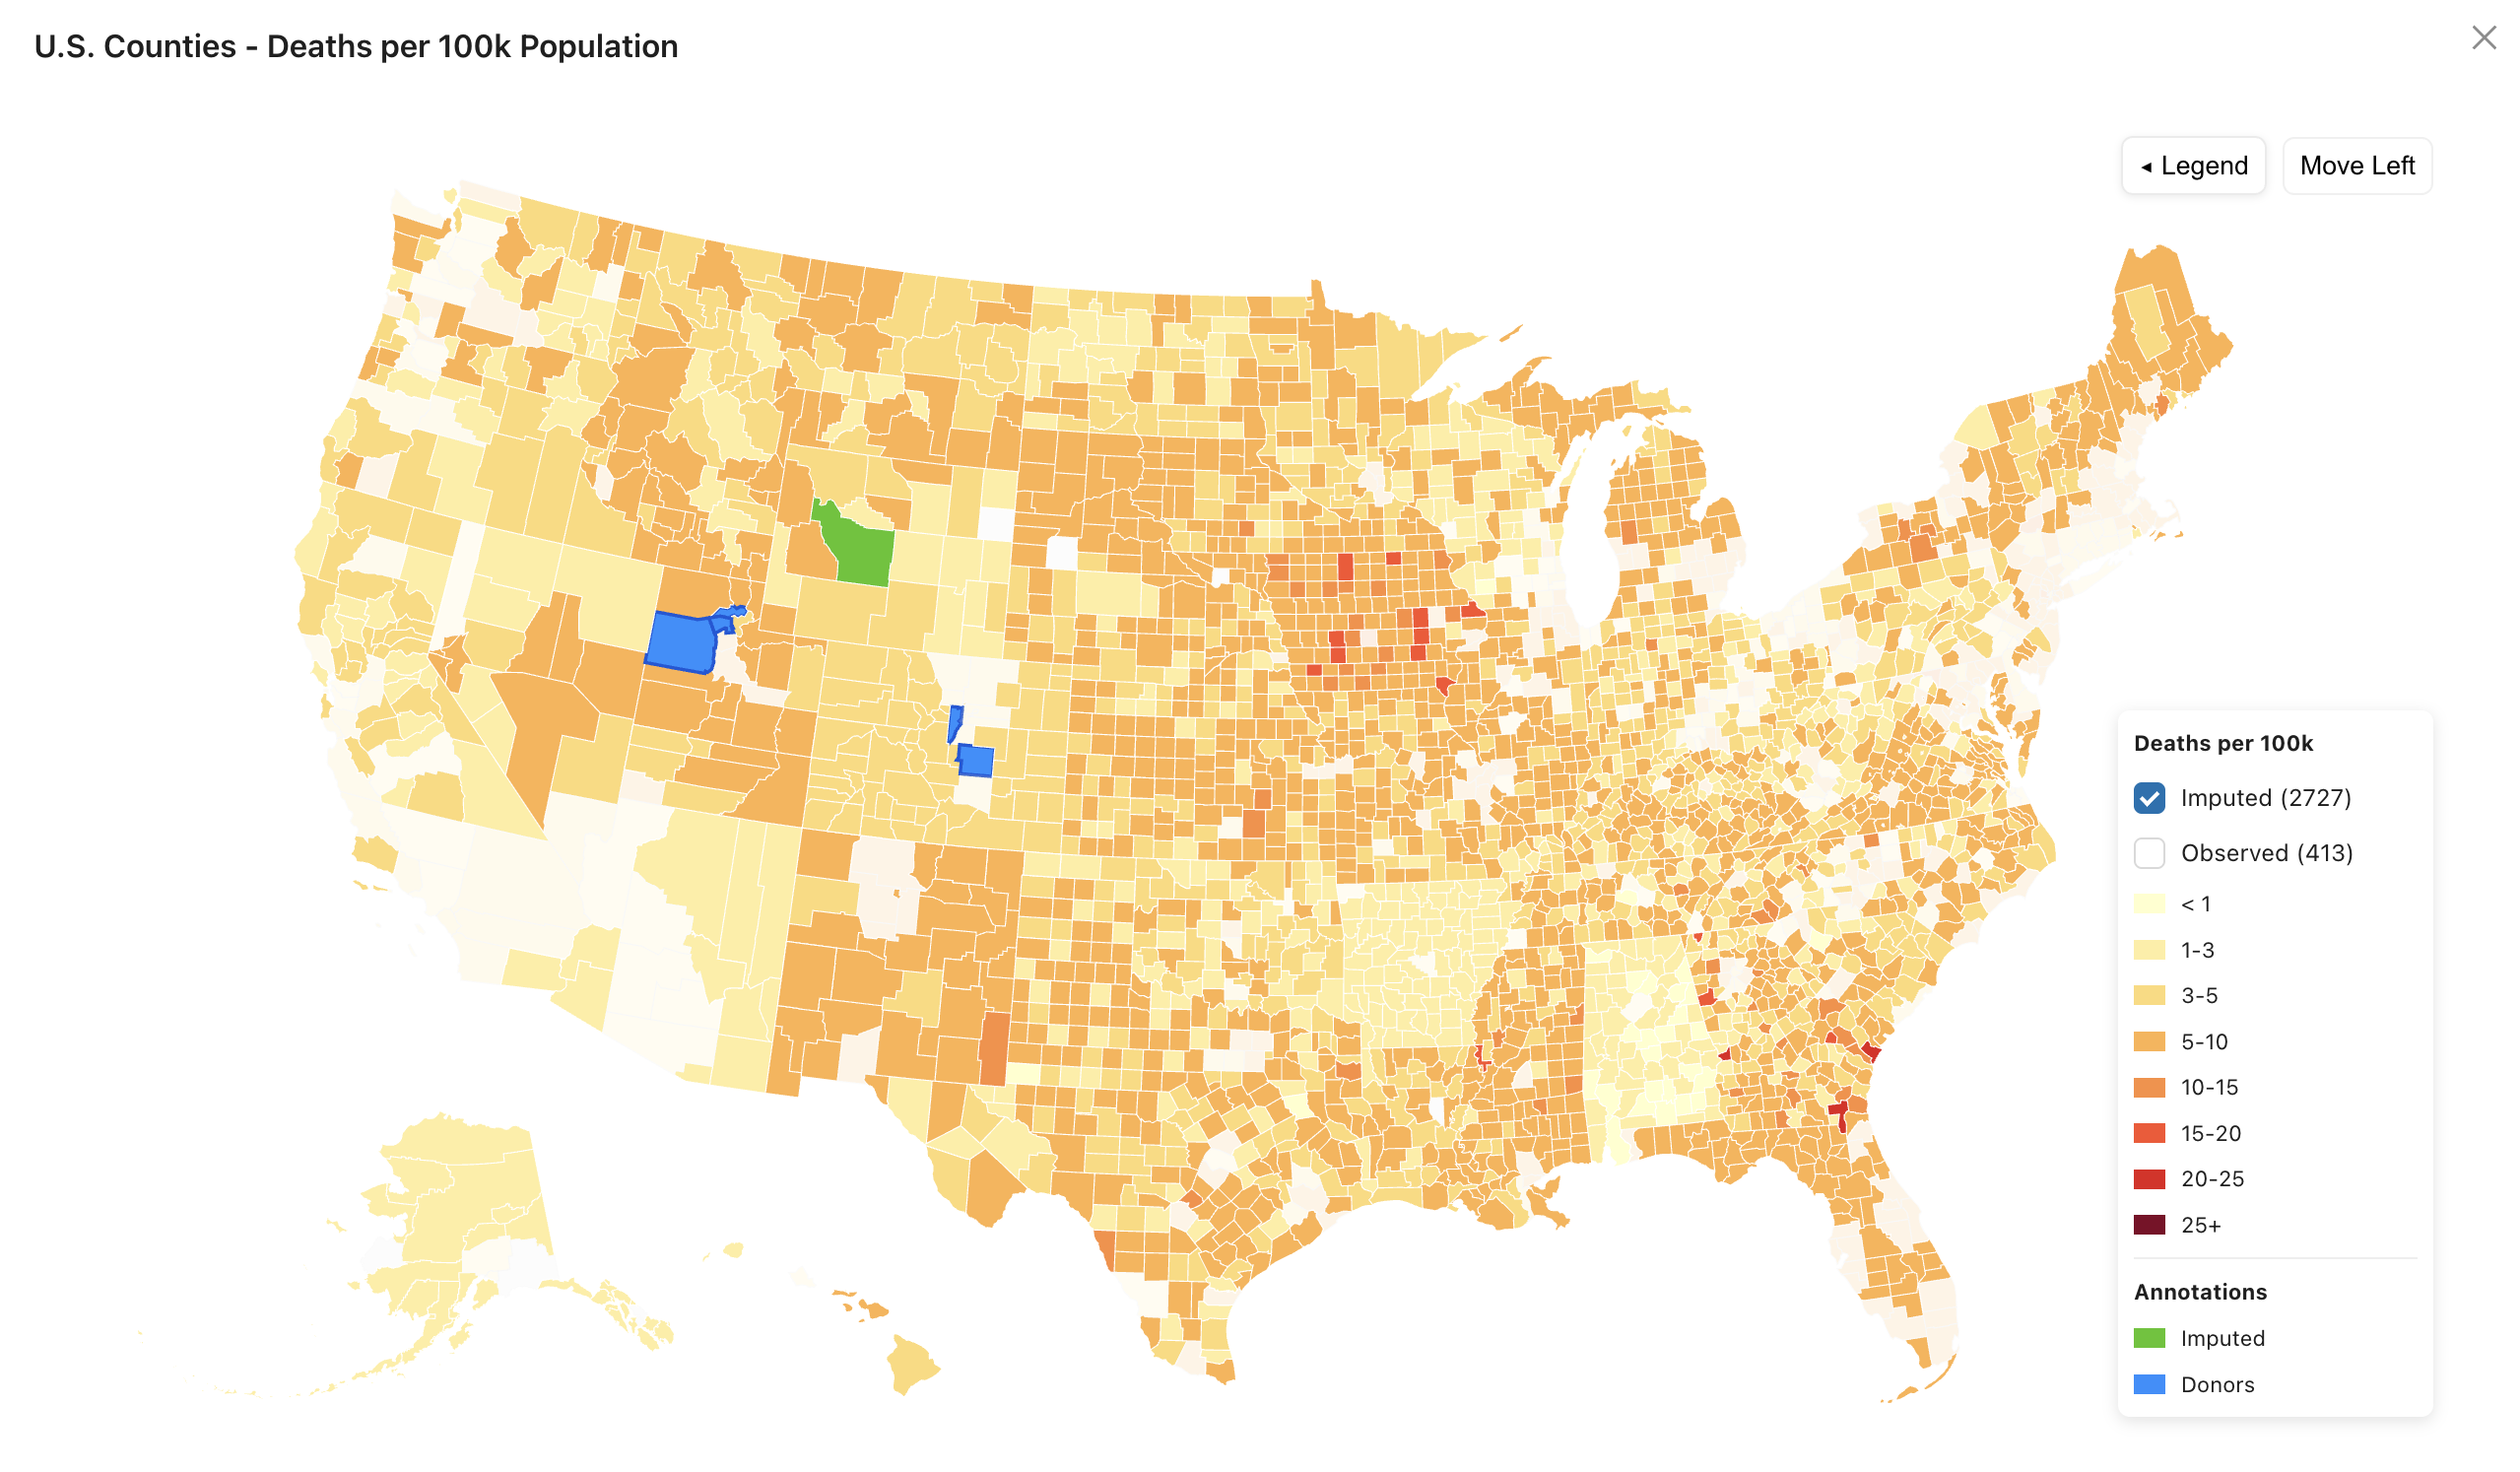
\includegraphics[width=\linewidth]{GeoMap.png}
  \caption{Figure: Geomap view for county-level opioid mortality with observed/imputed layer toggles and donor highlighting for selected imputed counties.}
  \label{fig:geomap_short}
\end{figure}

\section{Results}
\paragraph*{Accuracy across years and masks.}
\begin{table}[t]
  \centering
  \caption{Table: Average MAE (2000--2022) on prescription opioids across suppression-like (Supp.), intermediate (Interm.), random holdout (Random), and pooled Overall settings.}
  \label{tab:metrics}
  \begin{tabular}{@{}lcccc@{}}
    \toprule
    Method & Supp. & Interm. & Random & Overall \\
    \midrule
    Linear Regression & 4.07 & 2.91 & 2.88 & 3.28 \\
    kNN Regression    & 3.86 & 3.18 & 2.81 & 3.28 \\
    Random Forest     & 4.18 & 2.92 & 2.79 & 3.30 \\
    MICE              & 4.05 & 3.06 & 2.88 & 3.33 \\
    XGBoost           & 4.21 & 3.19 & 3.00 & 3.46 \\
    \textbf{\gknn}    & \textbf{3.47} & \textbf{2.76} & \textbf{2.66} & \textbf{2.96} \\
    \bottomrule
  \end{tabular}
\end{table}

Across 23 yearly opioid panels, \gknn achieves the lowest average MAE in all three masking regimes (Table~\ref{tab:metrics}), with strongest gains in suppression-like settings where geographic context is most informative. This indicates that integrating spatial proximity with socioeconomic similarity improves robustness when missingness is structurally tied to low-count regions.

\paragraph*{Case studies.}
In a 2010 opioid case study, paired Wilcoxon tests on per-county absolute errors indicate lower error for \gknn than non-spatial kNN (\(n=167\), mean difference \(-0.34\), \(p\approx0.0396\)). In the non-geographic telecom case, Random Forest clearly outperforms MICE (\(n=43\), mean difference \(21.9\), \(p\approx2.0\times10^{-9}\)), demonstrating that \tool supports data-appropriate model selection rather than favoring any single algorithm.

\begin{figure*}[t]
  \centering
  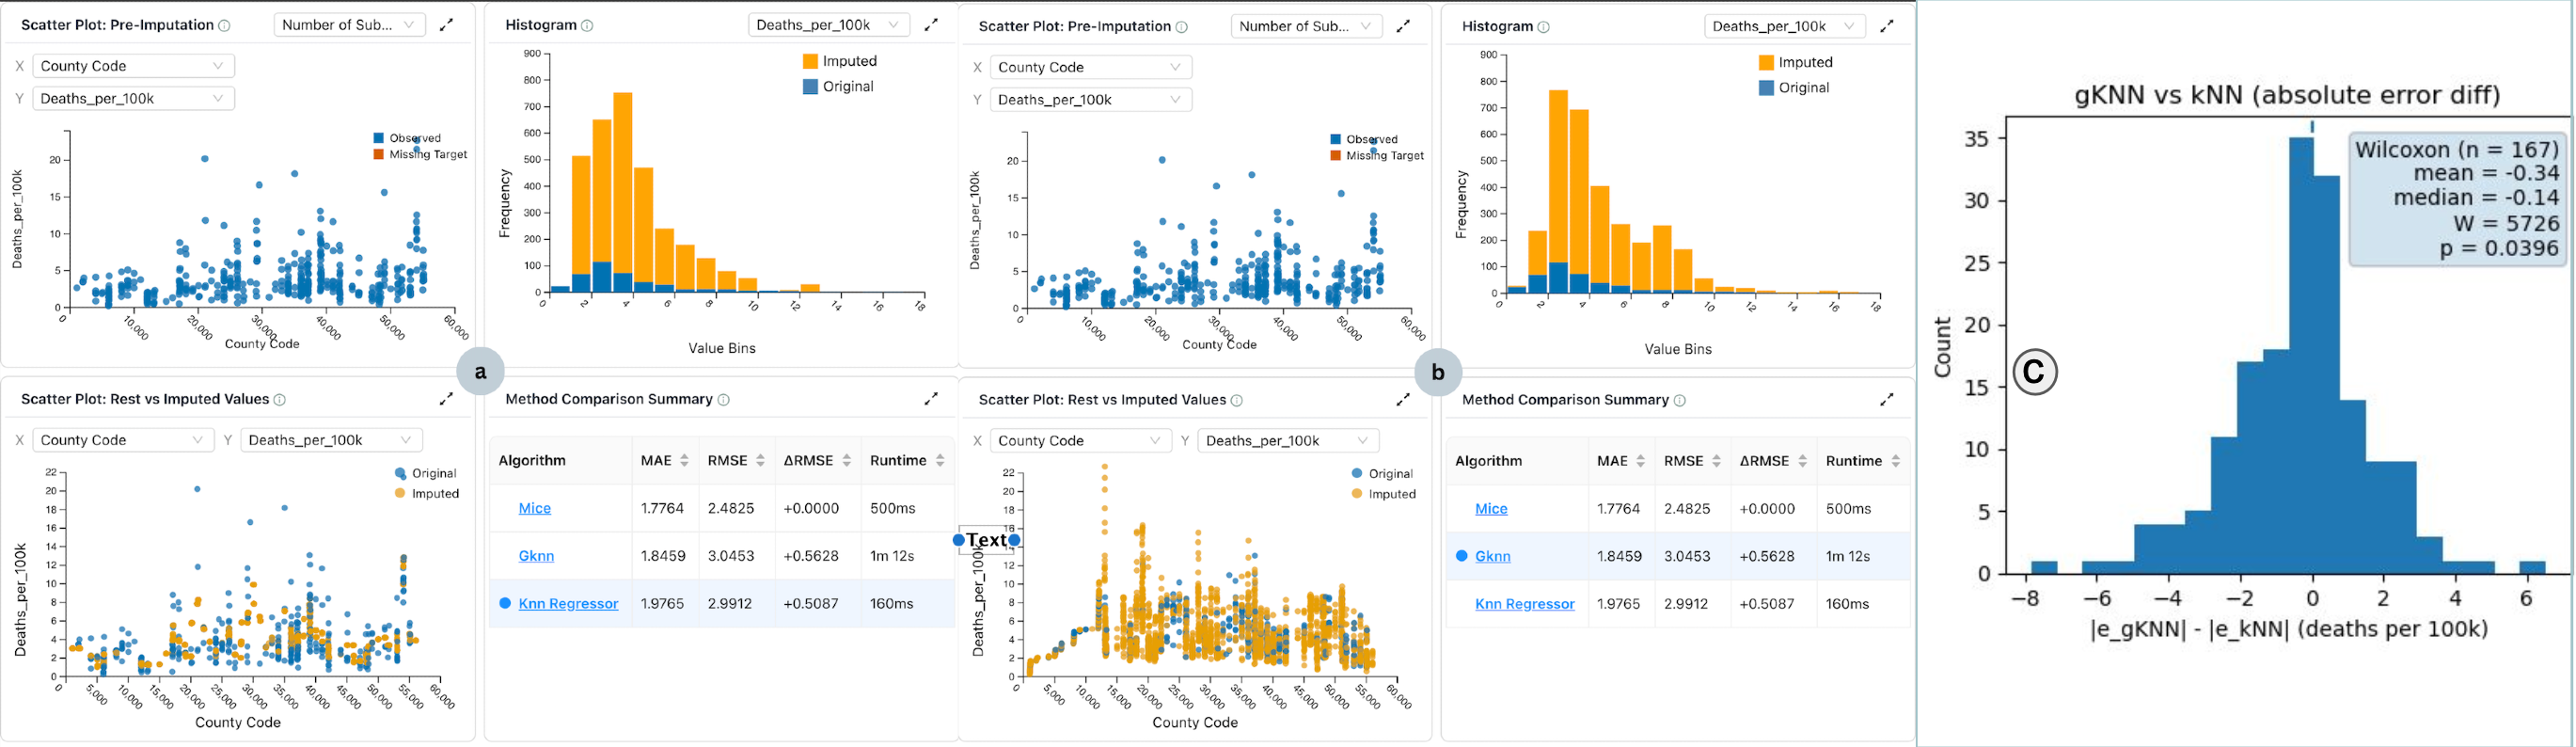
\includegraphics[width=\linewidth]{knn_gknn_wilcoxon.png}
  \caption{Figure: Spatial case study (2010 opioid mortality). Comparison of non-spatial kNN and \gknn, with distribution of per-county absolute-error differences. Most mass below zero indicates lower error for \gknn.}
  \label{fig:knn_gknn_short}
\end{figure*}

\paragraph*{Spatial case interpretation.}
In the opioid setting, the major qualitative difference between methods is donor geography. Baseline kNN can borrow from counties that are socioeconomically similar but spatially distant, which can over-smooth local hotspots. In contrast, \gknn tends to prioritize nearby counties with comparable profiles. Because donor sets are visible in the map and linked table, analysts can inspect whether each imputed estimate reflects plausible regional spillover or questionable long-range borrowing.

\subsection{Spatial opioid mortality: kNN vs gKNN}
The spatial opioid case highlights where geography changes conclusions. Under the same held-out mask, non-spatial kNN often smooths estimates toward broad socioeconomic averages, whereas \gknn better preserves localized regional variation by blending socioeconomic and geographic neighborhoods. In practice, this means counties with similar attributes but very different regional context are less likely to be treated as equivalent donors in \gknn.

The comparison is not only quantitative but operational: analysts can click imputed counties, inspect donor sets, and decide whether borrowing paths are epidemiologically plausible. This supports a key objective of the system---making imputation decisions inspectable rather than opaque. Even when MAE differences are moderate, provenance visibility helps determine whether errors are acceptable for downstream reporting tasks.

This behavior is particularly relevant in suppression-heavy regions where observed values are sparse. In such settings, pure feature-space neighbors may reflect demographic resemblance without reflecting local epidemic dynamics. By incorporating spatial proximity directly into the distance function, \gknn reduces these mismatches and tends to produce donor sets that align better with local context. The resulting improvement is visible not only in aggregate error but also in county-level residual patterns.

\subsection{Telecom churn: MICE vs Random Forest}
The telecom churn case provides a complementary non-geographic setting where spatial inductive bias is unnecessary. Using the same 20\% holdout strategy on the continuous \texttt{Offer} target, Random Forest consistently outperforms MICE. The per-row absolute-error differences favor Random Forest on most held-out records, and the paired Wilcoxon signed-rank test indicates a strong separation (\(n=43\), mean difference \(21.9\), \(p\approx2.0\times10^{-9}\)).

This case reinforces the system's method-agnostic intent. Rather than assuming a single best imputer, \tool allows analysts to identify when flexible non-linear tabular models dominate classical chained-equation approaches. In practice, users can validate this choice through the same linked diagnostics used in the spatial case, ensuring consistency in how evidence is gathered across domain types.

\section{Evaluation}
\subsection{Imputation accuracy}
Across yearly opioid panels and masking regimes, \gknn provides the strongest overall error profile in our benchmarked set (Table~\ref{tab:metrics}). Improvements are largest in suppression-like conditions, where missingness and geography are tightly coupled. This pattern supports the claim that explicitly modeling spatial context improves robustness when missingness is structurally tied to place.

At the same time, results across datasets reinforce that no single imputer is universally best. In non-geographic settings, tree-based models can outperform both \gknn and MICE, which is why \tool emphasizes side-by-side comparison under matched evaluation settings rather than fixed defaults. The method-comparison view therefore acts as a practical decision aid: it combines ranking signals (\(\Delta\)RMSE, MAE/RMSE, runtime) with linked distribution and relationship checks before analysts commit to exports.

We also note that performance differences are not uniform over years. In periods with stronger spatial concentration of overdose burden, gains from \gknn relative to non-spatial baselines are more pronounced; when spatial structure weakens, margins narrow and simpler models can become competitive. This temporal variability further motivates our design choice to keep all model outputs available for iterative comparison rather than relying on one static recommendation.

\subsection{Usability Evaluation}
In a formative usability study (\(N=7\)), the mean SUS score was 75.4 (SD 15.8), and participants rated method configurability and linked comparisons positively. Offline copula-based analysis for \gknn showed empirical coverage above 90\% across tested scenarios, with wider intervals under geography-only sampling, consistent with increased uncertainty when socioeconomic signal is excluded.

Task-level feedback indicates that users valued two aspects most: fast method switching with immediate visual updates, and donor-level explanations in the map workflow. Participants also reported that keeping axes stable across methods made comparisons easier and reduced re-interpretation effort. Lower ratings were concentrated around runtime latency and presentation polish, suggesting future improvements should focus on interaction smoothness and uncertainty cues rather than changes to core analytical functionality.

From a workflow perspective, participants tended to follow a repeatable sequence: diagnose missingness, run 2--3 candidate models, compare MAE/RMSE in the summary table, then inspect scatter/histogram/map views before choosing an export. This behavior aligns with our design goals and suggests the tool supports practical audit trails for method selection. Several participants explicitly noted that seeing donor provenance increased confidence when communicating results to non-technical stakeholders.

\paragraph*{Uncertainty analysis (summary).}
To complement holdout error, we use an offline copula-based analysis for \gknn to evaluate interval coverage and width under different conditional sampling assumptions. Coverage remains above 90\% in tested scenarios, while interval widening under geography-only conditioning reflects expected uncertainty when socioeconomic information is reduced. These results motivate future integration of lightweight uncertainty indicators directly into dashboard views.

\begin{figure}[t]
  \centering
  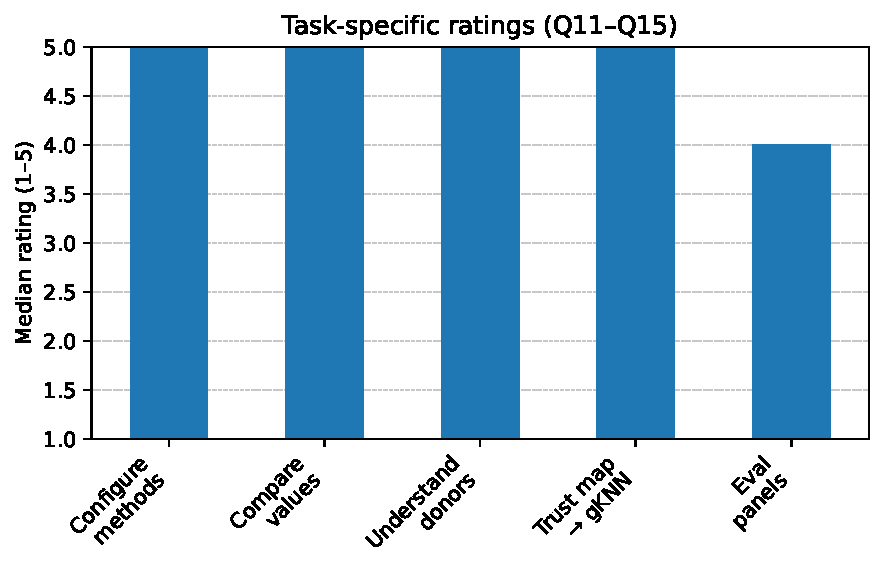
\includegraphics[width=0.95\linewidth]{usability_q11_15.pdf}
  \caption{Figure: Task-specific usability ratings (Q11--Q15) from the formative study.}
  \label{fig:usability_short}
\end{figure}

\section{Discussion and Conclusion}
\tool combines imputation execution, quantitative benchmarking, and provenance-rich visuals in a single workflow. The results show that spatially informed imputation improves accuracy when geographic autocorrelation is strong, while non-spatial models may dominate in purely tabular settings. This balance is central to the system design: it improves transparency and supports evidence-based model choice rather than algorithm lock-in.

Limitations include the current baseline set, computational cost of richer uncertainty analyses, and scalability constraints at finer geographic resolutions. Future work will extend algorithm coverage, integrate lighter-weight interactive uncertainty cues, and evaluate deployment in operational public-health analysis pipelines.
